\chapter{Literature review}
\label{cha:review}
\addcontentsline{toc}{chapter}{\MakeUppercase{Literature review}} 

\section{Introduction}

In the first chapter, the mathematical model of scanning electrochemical microscopy (SECM) redox-competition (RC-SECM) mode is presented for the first time in scientific research. The study is focused on solving systems of partial differential equations (PDEs) with nonlinear boundary conditions using numerical methods. Using this model, it is possible to calculate oxygen consumption rate, evaluate enzymatic reaction kinetics and determine oxygen diffusion coefficients in the medium of varying composition. Oxygen concentration measurement, which is important for SECM-based investigations of all biological systems, was successfully applied for the evaluation of enzymatic reaction performed by an immobilized enzyme. 

\section{Physical model} \label{sec:reakc_phys}

\subsection*{Reaction rate constants}  \label{subs:reakc_const}

In this research, the kinetic constants for reactions were gathered from references  and adjusted to better fit experimental results (Table \ref{tab:const}). Kinetic constants $k_{-1}$, $k_{-3}$, $k_{-4}$ for reactions were determined from the model and were set to the following values: $k_{-1} = \SI{10}{s^{-1}}$, $k_{-3} = \SI{2000}{M^{-1}s^{-1}}$. The constant $k_{-4}$ was set to zero, because the backward reaction is much slower than other reactions in diffusion-related processes. 

\begin{table}[ht!]
  \centering
  \caption{Kinetic constants and thermodynamic parameters for the GOx catalyzed reaction with $\beta$-D-glucose and oxygen at pH 5.5.}
  \label{tab:const}  
  \vspace{2mm} 
  \def\arraystretch{1.1}
  \begin{tabular}{ | m{8em} | c | c | c | c | c |}
    \hline
    Sugar substrate or thermodynamic parameter & \begin{tabular}{@{}c@{}} $k_{1}$,\\ \si{M^{-1}s^{-1}}\end{tabular} & $k_{2}$, \si{s^{-1}} & \begin{tabular}{@{}c@{}}  $k_{3}$,\\ \si{M^{-1}s^{-1}} \end{tabular} & $k_{4}$, \si{s^{-1}} & ref. \\ \hline
    %Sugar substrate or thermodynamic parameter & $k_{1}$, \si{M^{-1}s^{-1}} & $k_{2}$, \si{s^{-1}} & $k_{3}$, \si{M^{-1}s^{-1}} & $k_{4}$, \si{s^{-1}} & ref. \\ \hline
    $\beta$-D-glucose-1-\ce{^1H} at \SI{25}{\degreeCelsius} & ${\sim}200$ & ${\sim}\num{6000}$ & $\num{1.8d6}$ & $\num{1440}$ & \\ \hline
    $\beta$-D-glucose-1-\ce{^1H} at \SI{25}{\degreeCelsius} & $\num{13158}$ & & $\num{1.8d6}$ &  $\num{1440}$ & \\ \hline
    $\beta$-D-glucose-1-\ce{^1H} at \SI{27}{\degreeCelsius} & $\num{10000}$ & & $\num{2.1d6}$ & $\num{1150}$ & \\ 
\hline
    \midrule
    Used in the model & $\num{3000}$ & $\num{6000}$ & $\num{1.5d6}$ & $\num{1500}$ & \\ [1ex]
    \hline
  \end{tabular}
\end{table}


\section{Mathematical model}  \label{sec:reakc_math}

\begin{figure}[ht!]
\centering
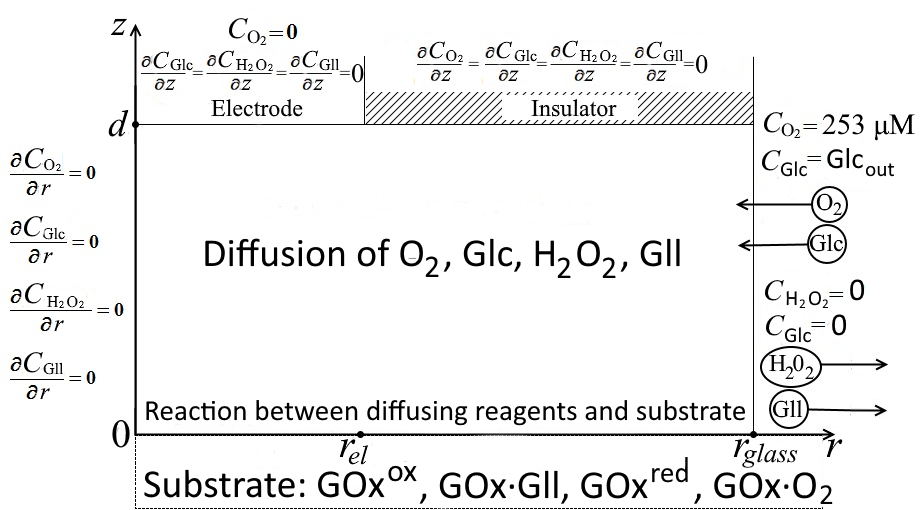
\includegraphics[width=1\linewidth]{chapter_1/Model_domain.png}
\caption{Scheme of simulation domain. All 8 reagents, boundary conditions for $C_{\text{diff}}$ and the direction of outside flux are displayed.}
\label{fig:Domain}
\end{figure}

Measurements of SECM acting in the redox-competition mode are changed into the scheme (\ref{fig:Domain}) due to the radial symmetry around the central axis of the electrode. Radial symmetry is a standard assumption in SECM modelling, though the case of off-centered UME was also investigated.

According to the second Fick’s law , diffusion processes are expressed by the system of partial differential equations (PDE):
\begin{equation}
  \begin{aligned}\label{eq:reakc_eq1}
  \frac{\partial C_{O_2}}{\partial t} &= D_{O_2}\,\Delta C_{O_2},\\
  \frac{\partial C_{Glc}}{\partial t} &= D_{Glc}\,\Delta C_{Glc},\\
  \frac{\partial C_{H_2 O_2}}{\partial t} &= D_{H_2 O_2} \,\Delta C_{H_2 O_2},\\
  \frac{\partial C_{Gll}}{\partial t} &= D_{Gll}\,\Delta C_{Gll},  \quad for\; 0<t\leq T,\; 0<z<d,\; 0<r<r_{glass},
  \end{aligned}
\end{equation}
where:
\begin{itemize}
  \item[] $C_{O_2}$, $C_{Glc}$, $C_{H_2 O_2}$ and $ C_{Gll}$ are concentrations of diffusing reagents and expressed as functions of time $t$ and spatial coordinates $z$ and $r$. Notation $C_{\text{diff}} = C_{\text{diff}} \left( t, z, r \right) = \left( C_{O_2}, C_{Glc}, \allowbreak C_{H_2 O_2}, \allowbreak C_{Gll} \right)$ was used when 4 diffusing re\-agents were considered together.
  \item[] $D_{O_2}$, $D_{Glc}$, $D_{H_2 O_2}$ and $D_{Gll}$ are diffusion coefficients of \ce{O2}, Glc, \ce{H2O2} and Gll.
  \item[] $d$ is the distance between the enzyme-modified surface and the electrode, which is varying from \SIrange{1}{120}{\um} as shown in Fig. \ref{fig:Domain}.
  \item[] $r_{glass} = \SI{80}{\um}$ is the radius of insulated area, $r_{el} = \SI{5}{\um}$ is the radius of electrode.
  \item[] $T$ is the duration of a computational experiment measured in seconds (the evaluation of this parameter is further explained in the next section).
  \item[] The Laplace operator $\Delta$ for concentration function $C$ in cylindrical coordinates with radial symmetry is
  \begin{equation*}
  \Delta C = \frac{1}{r}\frac{\partial }{\partial r} \left( r\frac{\partial C }{\partial r} \right) + \frac{\partial^{2} C}{\partial z^{2}}.
  \end{equation*}
\end{itemize}

